\usetikzlibrary{arrows.meta,chains,fit,matrix}
\begin{frame}<all:1-7,10,8-9>[fragile,label=ptInMem1]{page tables in memory}
\begin{itemize}
\item where can processor store megabytes of page tables? \myemph{in memory}
\end{itemize}
% FIXME: big page table picture marked in memory with memory addresses
%         and page table base register

% FIXME: animation
\begin{tikzpicture}
\tikzset{
    every node/.style={font=\fontsize{10}{11}\selectfont},
    >=Latex,
}
% page table entry layout
\matrix[anchor=south,tight matrix,nodes={draw,minimum height=0.4cm,text width={}},label={north:page table entry layout}]
    at (8, 3){
        |[alt={<all:4,8>{red}}]| valid (bit 15) \& |[alt=<all:5>{red}]| kernel (bit 14) \& |[alt={<all:6,9>{red}}]| physical page \# (bits 4--13) \& unused (bit 0-3) \\
};

\begin{visibleenv}<all:7->
\matrix[tight matrix,anchor=north west,
        nodes={text width=2.3cm,minimum height=0.3cm,font=\fontsize{10}{11}\selectfont\tt,black!80},
        column 1/.style={nodes={draw=none,align=right}},
        column 2/.style={nodes={draw,thick,text width=1.2cm,align=center,alt=<all:8>{red}}},
        column 3/.style={nodes={draw,thick,text width=1.2cm,align=center}},
        column 4/.style={nodes={draw,thick,text width=2.7cm,alt=<all:9>{red}}},
        row 1/.style={nodes={draw=none,font=\fontsize{10}{11}\selectfont\normalfont}},
        label={above:page table (logically)},
    ] (pt) at (0, 0) {
    virtual page \# \& valid? \& kernel? \& physical page \# \\
    0000 0000 \& 0 \& 0 \& 00 0000 0000 \\
    0000 0001 \& 1 \& 0 \& 10 0010 0110\\
    0000 0010 \& 1 \& 0 \& 00 0000 1100 \\
    0000 0011 \& 1 \& 0 \& 11 0000 0011 \\
    \ldots \\
    1111 1111 \& 1 \& 0 \& 00 1110 1000 \\
};
\end{visibleenv}

\begin{visibleenv}<all:3->
\matrix[tight matrix,anchor=north west,
        nodes={text width=2.8cm,minimum height=0.3cm,font=\fontsize{10}{11}\selectfont\tt},
        column 1/.style={nodes={draw=none,align=right}},
        column 2/.style={nodes={draw,thick,text width=3.75cm,align=center}},
        row 1/.style={nodes={draw=none}},
        label={above:physical memory},
    ] (pm) at ([xshift=1cm,yshift=2cm]pt.north east){
    addresses \& bytes \\
    0x00000000-1 \& 00000000 00000000 \\
    \ldots \\
    0x00010000-1 \& \myemph<all:4,8>{0}\myemph<all:5>{0}\myemph<all:6,9>{000000 0000}0000 \\
    0x00010002-3 \& \myemph<all:8>{1}0\myemph<all:9>{100010 0110}0000 \\
    0x00010004-5 \& \myemph<all:8>{1}0\myemph<all:9>{000010 1100}0000 \\
    0x00010006-7 \& \myemph<all:8>{1}0\myemph<all:9>{110000 0011}0000 \\
    \ldots \\
    0x000101FE-F \& \myemph<all:8>{1}0\myemph<all:9>{001110 1000}0000 \\
    0x00010200-1 \& 10100010 00111010 \\
};
\end{visibleenv}

\begin{visibleenv}<all:2->
\node[draw,very thick,above=1cm of pt,label={north:page table base register},xshift=-1.5cm] (ptbr) {\tt 0x00010000};
\draw[->,very thick,dashed] (ptbr) |- (pm-4-1);
\end{visibleenv}

\begin{visibleenv}<all:7->
    \draw[dotted,<->] (pm-4-1.west) -- (pt-2-4.east);
    \draw[dotted,<->] (pm-5-1.west) -- (pt-3-4.east);
    \draw[dotted,<->] (pm-6-1.west) -- (pt-4-4.east);
    \draw[dotted,<->] (pm-9-1.west) -- (pt-7-4.east);
\end{visibleenv}

\end{tikzpicture}
\end{frame}

\begin{frame}<all:1-8>{memory access with page table}
\begin{tikzpicture}
\tikzset{
    >=Latex,
    pageNumber/.style={fill=blue!10,font=\fontsize{11}{12}\selectfont,inner sep=.5mm},
    pageOffset/.style={fill=green!10,font=\fontsize{11}{12}\selectfont,inner sep=.5mm},
    comp/.style={fill=yellow!10,font=\fontsize{12}{13}\selectfont},
    memAccess/.style={alt=<7>{red, very thick}},
}
\node[pageNumber] (addrLeft) {11 0101 01};
\node[anchor=west,pageOffset] (addrRight) at (addrLeft.east) {00 1101 1111};
\begin{visibleenv}<2->
\node[draw,comp,below=1cm of addrLeft] (timesPte) {$\times$ PTE size};
\draw[->,thick] (addrLeft) -- (timesPte);
\node[draw,very thick,below left=3cm and 1cm of addrLeft,label={[align=center]north:page table\\base register}] (ptbr) {\tt 0x10000};
\node[draw,comp] (plus) at (timesPte.south |- ptbr.west) {+};
\draw[->,thick] (timesPte) -- (plus);
\draw[->,thick] (ptbr) -- (plus);
\end{visibleenv}

\begin{visibleenv}<3->
\node[below=2cm of plus,fill=violet!10,draw,very thick,minimum height=1cm,minimum width=12cm,xshift=3cm] (cache) {data or instruction cache};
\node[pageNumber] (addrLeftFinal) at ([xshift=7cm]plus) {1101 0011 11};
\draw[->,thick,memAccess] (plus) -- (cache.north -| plus.south);
\node[above right=1cm and 2cm of plus,align=center,draw,comp] (check) {check valid \\ and kernel bit};
\node[below=1cm of check,draw,comp] (split) {split PTE parts};
\draw[->,thick] (cache.north -| split.south) -- (split.south);
\draw[->,thick] (split) -- (check);
\draw[->,thick] ([xshift=1cm]check.north) -- ++(1cm, 1cm) node[above] {cause fault?};
\draw[blue!50!black,->,thick] (split) -- (addrLeftFinal);
\end{visibleenv}

\begin{visibleenv}<4->
\node[anchor=west,pageOffset] (addrRightFinal) at (addrLeftFinal.east) {00 1101 1111};
\draw[very thick,green!50!black,densely dotted] (addrRight) |- ([xshift=-.5mm,yshift=.5cm]split.north);
\draw[very thick,green!50!black,densely dotted,->] ([xshift=.5mm,yshift=.5cm]split.north) -| (addrRightFinal.north);
\end{visibleenv}
\begin{visibleenv}<3->
\node[inner sep=0mm,draw,label={[font=\fontsize{12}{13}\selectfont]south:physical address},fit=(addrLeftFinal) (addrRightFinal)] (addrFinal) {};
\end{visibleenv}

\node[inner sep=0mm,draw,label={[font=\fontsize{12}{13}\selectfont]north:virtual address},fit=(addrLeft) (addrRight)] (addr) {};
\begin{visibleenv}<5->
    \draw[->,thick,memAccess] (addrFinal) -- (cache.north -| addrFinal.south);
\end{visibleenv}

\begin{pgfonlayer}{bg}
\begin{visibleenv}<6->
    \node [fill=black!5,fit=(timesPte) (split),draw,line width=0.5mm,dashed,label={south:memory management unit (MMU)}] (mmu) {};
\end{visibleenv}
\end{pgfonlayer}

\begin{visibleenv}<7>
    \node[fill=white,draw=red,ultra thick,align=center] at ([xshift=1cm]mmu.center) {
        one program cache/memory access becomes \\
        multiple cache/memory accesses
    };
\end{visibleenv}

\end{tikzpicture}
\end{frame}

\begin{frame}{MMUs in the pipeline}
% FIXME: CPU pipeline stages with MMU and caches
% FIXME: diagram of memory access
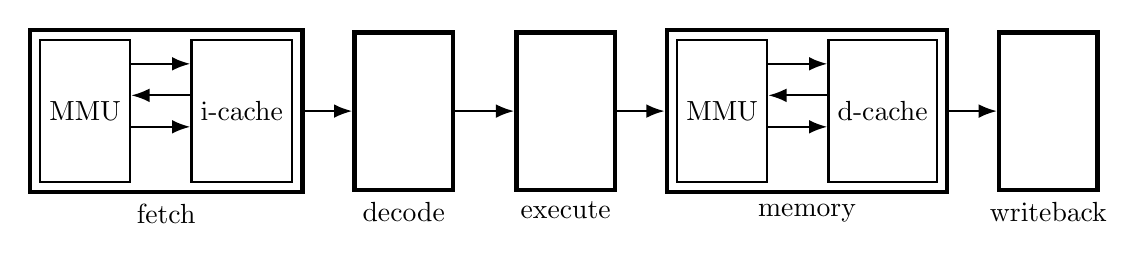
\begin{tikzpicture}
\tikzset{
    stage/.style={draw,ultra thick,minimum height=2cm,minimum width=1.25cm,font=\small},
    subStage/.style={draw,thick, minimum height=1.8cm,font=\fontsize{10}{11}\selectfont},
    >=Latex,
}

\begin{scope}[start chain=going right,every join/.style={->,thick},node distance=7.5mm]
\node[subStage,on chain] (immu) {MMU};
\node[subStage,on chain=going right] (icache) {i-cache};
\node[stage,on chain,label={south:decode}] (decode) {};
\node[stage,on chain,label={south:execute}] (execute) {};
\node[subStage,on chain] (dmmu) {MMU};
\node[subStage,on chain] (dcache) {d-cache};
\node[stage,on chain,label={south:writeback}] (writeback) {};
\end{scope}
\foreach \x in {2mm} {
    \draw[<-,thick] ([yshift=\x]immu.east) -- ([yshift=\x]icache.west);
    \draw[<-,thick] ([yshift=\x]dmmu.east) -- ([yshift=\x]dcache.west);
}
\foreach \x in {6mm,-2mm} {
    \draw[->,thick] ([yshift=\x]immu.east) -- ([yshift=\x]icache.west);
    \draw[->,thick] ([yshift=\x]dmmu.east) -- ([yshift=\x]dcache.west);
}
\node[stage,fit=(immu) (icache),label={south:fetch}] (fetch) {};
\node[stage,fit=(dmmu) (dcache),label={south:memory}] (memory) {};
\draw[->,thick] (fetch) -- (decode);
\draw[->,thick] (decode) -- (execute);
\draw[->,thick] (execute) --  (memory);
\draw[->,thick] (memory) -- (writeback);
\end{tikzpicture}
\begin{itemize}
\item \myemph{up to four memory accesses} per instruction
\item<2-> challenging to make this fast (topic for a future date)
\end{itemize}
\end{frame}
